\secnumbersection{PROPUESTA DE SOLUCIÓN}
\setcounter{secnumdepth}{4}
\setcounter{tocdepth}{4}
\makeatletter
\renewcommand\paragraph{\@startsection{paragraph}{4}{\z@}%
  {1.5ex \@plus .5ex \@minus .2ex}%   % espacio antes
  {0.8ex \@plus .2ex}%                 % espacio después
  {\normalfont\normalsize\bfseries}}  % estilo
\makeatother



Esta propuesta abarca la evolución de \textbf{DRAFTS} \cite{zhang2024drafts} desde un prototipo de investigación para la detección y clasificación de FRBs, hacia un \textit{pipeline} 
\textbf{productivo, robusto y eficiente} diseñado para detectar y clasificar transientes de radio y FRBs de forma sencilla y fácil para el astrónomo. Esta transformación arquitectónica no se limita a 
mejoras incrementales, sino que además establece una \textbf{extensión fundamental para regímenes de alta frecuencia} que expande significativamente las capacidades de 
detección en el espectro milimétrico.

De ahora en adelante, a esta nueva versión de DRAFTS le llamaremos DRAFTS++, que es básicamente toda esta memoria.

\subsection{Vista General: Dos Grandes Bloques de Contribución a los pipelines astronómicos de FRBs}

Esta propuesta se estructura en \textbf{dos grandes bloques} que abordan desafíos complementarios en la detección de FRBs:

\begin{itemize}
    \item \textbf{Bloque 1: DRAFTS++: Pipeline astronómico E2E, Productivo, Robusto y Eficiente}: Este bloque aborda la transformación del prototipo DRAFTS hacia un sistema productivo capaz de operar en entornos observacionales reales. Este bloque incluye la refactorización arquitectónica completa; la implementación de procesamiento eficiente por \emph{chunks}; la gestión eficiente de memoria y recursos; la trazabilidad completa; y artefactos de salida estandarizados.

    \item \textbf{Bloque 2: DRAFTS++: Extensión a Alta Frecuencia - Cuatro Líneas de Investigación:} Este bloque explora estrategias metodológicas para extender las capacidades de detección hacia regímenes de alta frecuencia (30-100 GHz), donde las firmas dispersivas tradicionales se atenúan significativamente. Este bloque presenta cuatro líneas de investigación complementarias que abordan diferentes aspectos del desafío de detección en el espectro milimétrico.
\end{itemize}

\subsection{Bloque 1: DRAFTS++: Pipeline astronómico E2E, Productivo, Robusto y Eficiente}

Como ya se mencionó anteriormente, aquí se contempla la transformación fundamental del prototipo DRAFTS hacia un sistema productivo capaz de operar en entornos observacionales reales. La evolución desde un prototipo de investigación hacia un sistema productivo requiere una transformación arquitectónica fundamental que aborde las limitaciones inherentes del código base original.

\subsubsection{Desafíos y limitaciones de DRAFTS}

DRAFTS es un "pseudo-pipeline", mas cerca a ser un prototipo que un software astronomico, pero ojo, en cuanto a lo que son los modelos de redes neuronales estos son modelos de deteccion y clasificacion de FRBs robustos y completamente funcionales, el problema surge al rededor de estos modelos, pues DRAFTS presenta una estructura monolítica con scripts independientes optimizados para condiciones de laboratorio controladas pero incapaces de manejar la variabilidad operacional de entornos observacionales reales. Más que limitaciones incrementales, el código original no constituye un \emph{pipeline} operativo: la búsqueda en datos reales se materializa en programas separados que el usuario debe ejecutar y parametrizar manualmente. No existe un punto de entrada unificado, una interfaz de línea de comandos ni un sistema de configuración versionado; el flujo exige editar variables en el código (rutas, umbrales, \textit{checkpoints}, tamaños de bloque, DM, etc.) y correr etapas desconectadas sin orquestación. El propio \texttt{README} instruye a “modificar la ruta de datos y de guardado y ejecutar el archivo”, lo que evidencia la ausencia de un flujo automatizado de extremo a extremo que, con un único \emph{input}, entregue resultados reproducibles, directos y simples para el usuario astrónomo.

En la ingesta de datos se observan supuestos instrumentales rígidos. El lector de PSRFITS asume un esquema específico propio de FAST/GBT, y el repositorio indica explícitamente que para otros telescopios se deben “modificar” funciones internas. No hay detección automática de formato ni un análisis robusto de encabezados; los parámetros observacionales se derivan parcialmente con constantes implícitas y números mágicos (p.ej., factores de decimado temporal y espectral), además de correcciones ad hoc como la inversión del eje de frecuencia o normalizaciones mín--máx. Tampoco se calculan marcas temporales precisas a partir de los \emph{headers}, por lo que los tiempos de arribo son relativos y no trazables de manera consistente dentro del archivo ni interoperables con análisis posteriores.

La gestión de datos y memoria es frágil para observaciones prolongadas. El procesamiento es monolítico sobre bloques grandes construidos concatenando archivos contiguos en memoria, y para completar las ventanas de dedispersión en los bordes se recurre a relleno sintético con ruido aleatorio cuando faltan muestras, alterando la estadística de fondo y comprometiendo la validez científica en condiciones reales. La dedispersión GPU (\texttt{numba.cuda}) opera sobre tensores completos de DM--tiempo sin un planificador de \textit{chunking} que respete un presupuesto de memoria; no hay telemetría ni control de uso de VRAM, limpieza sistemática, \textit{fallback} a CPU ante \emph{out-of-memory} o manejo robusto de errores. Esta combinación limita la estabilidad y escalabilidad del sistema cuando la duración, el ancho de banda o la resolución crecen.

La extracción y validación de candidatos carecen de un esqueleto unificado. La detección obtiene cajas en DM--tiempo, pero el filtrado posterior es heurístico (p.ej., exigir \texttt{DM > 20}) y la clasificación está desacoplada en un programa distinto que dedispersa a un DM fijo predefinido, sin realimentación del detector. No existe un validador físico común (coherencia por sub--bandas, verificación de DM positivo con incertidumbre acotada, consistencia temporal entre ventanas) ni mecanismos de desduplicación de eventos entre \emph{slices} y archivos. Las salidas se limitan a imágenes y algunos archivos \texttt{.npy} por bloque; no se generan artefactos estandarizados (CSV/Parquet con metadatos completos), ni resúmenes por ejecución, ni firmas de modelos y datos que habiliten trazabilidad y auditoría. La ausencia de \emph{logging} estructurado y de semillas controladas impide reproducir resultados de manera fiable.

En operación y extensibilidad, los modelos se cargan desde rutas relativas y su presencia es un prerrequisito tácito; si faltan, el programa simplemente falla sin orientación al usuario. No hay empaquetado ni instalación como librería, pruebas automatizadas, ni documentación de un flujo end--to--end; el entrenamiento existe, pero la integración con la búsqueda es manual. La compatibilidad multi--banda y el tratamiento de polarización son limitados (se promedian canales y polarizaciones tempranamente), y no existe un mecanismo para seleccionar estrategias de búsqueda según condiciones físicas (resolución temporal, rango de frecuencias, SNR, disponibilidad de Stokes). 

En suma, a pesar de contar con modelos de detección y clasificación bien entrenados, el prototipo carece del software de \emph{pipeline} que permita, con un único \emph{input}, obtener resultados directos, sencillos y trazables en un entorno observacional real, es de ahi que nace DRAFTS++.

\subsubsection{Construccion de un Pipeline End-to-End Modular y Escalable: DRAFTS++}

A continuación, se procede a explicar y narrar la transformación arquitectónica fundamental que sufrió DRAFTS para ser DRAFTS++. 

La evolución desde los scripts monolíticos hacia un sistema modular escalable constituye una contribución arquitectónica fundamental que establece las bases para operaciones productivas a gran escala. Esta transformación implementa una arquitectura modular con componentes especializados que establecen separación clara de responsabilidades e interfaces estandarizadas. La reestructuración arquitectónica elimina las limitaciones inherentes del prototipo original, caracterizado por scripts independientes sin integración coherente, y establece un flujo de datos unidireccional que garantiza consistencia operacional y facilita mantenimiento y extensibilidad del sistema.

Para materializar todo esto, DRAFTS++ se gestiona en \textbf{etapas encadenadas} que transforman los datos desde la ingesta hasta los artefactos finales, y en \textbf{servicios transversales} que aseguran orden, reproducibilidad y operación continua. Las etapas (ingesta, preprocesamiento, modelos, detección, análisis y visualización) reciben entradas bien definidas y devuelven salidas contratadas; los transversales (\texttt{core/}, \texttt{config/}, \texttt{logging/}, \texttt{scripts/}) proveen orquestación, configuración validada, trazabilidad y puntos de entrada. Este enfoque divide el problema en unidades comprensibles y sustituibles, habilitando evolución independiente sin comprometer la coherencia global.

La \textbf{visión operativa} se resume en cuatro ejes: (i) un uso \textbf{productivo} del sistema, con punto de entrada único, configuración centralizada y artefactos estandarizados; (ii) \textbf{robustez} frente a formatos y condiciones instrumentales diversas mediante autodetección, validaciones físicas/temporales y recuperación guiada ante fallos; (iii) \textbf{eficiencia} por streaming con presupuestos de memoria explícitos, limpieza determinística y uso controlado de GPU; y (iv) \textbf{replicabilidad/auditoría} garantizada por semillas fijas, versiones y firmas de datos/modelos y \emph{logging} estructurado.

Para sostener estos ejes se adoptan \textbf{principios arquitectónicos} claros: modularidad y separación de responsabilidades; flujo de datos estrictamente unidireccional con \textbf{contratos} entre etapas (geometrías, metadatos, candidatos); configuración validada con valores por defecto seguros; \textbf{streaming y \emph{chunking}} con solapamiento físico y continuidad temporal verificada; \textbf{observabilidad} mediante métricas y estados normalizados; y \textbf{outputs estandarizados} que facilitan consumo externo y auditoría científica.

Para entender mejor esto, podemos ver la Figura \ref{fig:workflow-src}, la cual resume el flujo principal y los soportes transversales del pipeline DRAFTS++, que guían el orden de este Bloque 1.

\begin{figure}[H]
\centering
\begingroup\shorthandoff{<>}% desactivar atajos de babel para < y > dentro de TikZ
\resizebox{\textwidth}{!}{%
\begin{tikzpicture}[
    node distance=1.0cm and 1.6cm,
    stage/.style={rectangle, draw, fill=blue!20, text width=2.7cm, text centered, minimum height=0.7cm, font=\small},
    support/.style={rectangle, draw, fill=gray!20, text width=2.7cm, text centered, minimum height=0.6cm, font=\small, rounded corners},
    arrow/.style={-Stealth, thick, shorten >=2pt}
]

% Flujo principal por etapas (de izquierda a derecha)
\node[stage] (in) {input/\\Ingesta};
\node[stage, right=of in] (pp) {preprocessing/\\Preprocesamiento};
\node[stage, right=of pp] (md) {models/\\Modelos};
\node[stage, right=of md] (dt) {detection/\\Detección};
\node[stage, right=of dt] (an) {analysis/\\Análisis};
\node[stage, right=of an] (vz) {visualization/\\Visualización};
\node[stage, right=of vz] (out) {output/\\Artefactos};

\draw[arrow] (in) -- (pp);
\draw[arrow] (pp) -- (md);
\draw[arrow] (md) -- (dt);
\draw[arrow] (dt) -- (an);
\draw[arrow] (an) -- (vz);
\draw[arrow] (vz) -- (out);

% Módulos transversales de soporte (debajo)
\node[support, below=3.2cm of md] (core) {core/\\Utilidades y Orquestación};
\node[support, left=1.8cm of core] (cfg) {config/\\Configuración};
\node[support, right=1.8cm of core] (log) {logging/\\Registro};
\node[support, below=2.2cm of core] (scr) {scripts/\\CLI y Entradas};

% Conexiones (líneas punteadas) desde soporte a etapas
% Conexiones (desde borde superior de soporte al borde inferior de etapas)
\draw[arrow, dashed] (core.north) -- (in.south);
\draw[arrow, dashed] (core.north) -- (pp.south);
\draw[arrow, dashed] (core.north) -- (md.south);
\draw[arrow, dashed] (core.north) -- (dt.south);
\draw[arrow, dashed] (core.north) -- (an.south);
\draw[arrow, dashed] (core.north) -- (vz.south);

\draw[arrow, dashed] (cfg.north) -- (in.south);
\draw[arrow, dashed] (cfg.north) -- (pp.south);
\draw[arrow, dashed] (cfg.north) -- (md.south);
\draw[arrow, dashed] (cfg.north) -- (dt.south);
\draw[arrow, dashed] (cfg.north) -- (an.south);
\draw[arrow, dashed] (cfg.north) -- (vz.south);

\draw[arrow, dashed] (log.north) -- (md.south);
\draw[arrow, dashed] (log.north) -- (dt.south);
\draw[arrow, dashed] (log.north) -- (an.south);

\draw[arrow, dashed] (scr.north) -- (in.south);
\draw[arrow, dashed] (scr.north) -- (pp.south);
\draw[arrow, dashed] (scr.north) -- (md.south);
\draw[arrow, dashed] (scr.north) -- (dt.south);
\draw[arrow, dashed] (scr.north) -- (an.south);
\draw[arrow, dashed] (scr.north) -- (vz.south);

\end{tikzpicture}}
\endgroup
\caption{Arquitectura modular del pipeline DRAFTS++ basada en la estructura de carpetas en \texttt{src/}: flujo principal (ingesta $\to$ preprocesamiento $\to$ modelos $\to$ detección $\to$ análisis $\to$ visualización $\to$ artefactos) y módulos transversales de soporte (\texttt{core/}, \texttt{config/}, \texttt{logging/}, \texttt{scripts/}). Esta figura introduce la construcción de DRAFTS++ como pipeline productivo y eficiente, sin incluir aún la extensión de alta frecuencia.}
\label{fig:workflow-src}
\end{figure}

A continuación se presentarán, de manera secuencial y detallada, cada una de estas etapas, para facilitar la comprensión de las mejoras implementadas.

\subsubsection{Ingesta multi-formato y análisis automático}

La ingesta de datos constituye la primera etapa crítica del pipeline, donde se establece la base para todo el procesamiento posterior. DRAFTS++ implementa un sistema de ingesta completamente automatizado que elimina las limitaciones instrumentales rígidas del prototipo original, proporcionando detección automática de archivos, manejo robusto de múltiples formatos y análisis inteligente de parámetros observacionales.

\paragraph{Detección automática de archivos astronomicos}

El sistema de detección automática implementado en un modulo, transforma la búsqueda manual de archivos en un proceso completamente automatizado. A diferencia del prototipo original de DRAFTS que requiere especificación manual de rutas y archivos individuales, DRAFTS++ implementa algoritmos que escanean directorios de datos y detectan automáticamente archivos compatibles basándose en el objetivo FRB especificado.

El algoritmo de búsqueda opera mediante filtrado inteligente por nombre de archivo, identificando automáticamente archivos FITS y Filterbank que contienen el objetivo especificado en su nombre. Esta aproximación elimina la necesidad de especificar rutas manualmente y reduce significativamente los errores humanos en la selección de archivos para procesamiento. El sistema proporciona logging estructurado que reporta el número de archivos encontrados por tipo, facilitando la validación y monitoreo del proceso de ingesta.

La validación automática de compatibilidad implementada verifica la integridad y compatibilidad de cada archivo antes del procesamiento, detectando archivos corruptos, vacíos o con formatos no soportados. Esta validación previene fallos tardíos durante el procesamiento y proporciona mensajes de error informativos que facilitan la resolución de problemas.

\paragraph{Manejo robusto de formatos FITS y Filterbank}

La implementación de parsers especializados para múltiples formatos astronómicos constituye una mejora fundamental que elimina las limitaciones instrumentales específicas del prototipo original. DRAFTS++ implementa bloques de codigos controladores que proporcionan manejo nativo y optimizado para formatos PSRFITS, FITS estándar y SIGPROC Filterbank.

El parser FITS maneja automáticamente las diferencias entre implementaciones de telescopios específicos, incluyendo correcciones de orden de frecuencia, normalizaciones específicas y manejo de diferentes esquemas de polarización. La implementación incluye detección automática de formatos de datos (1-bit, 8-bit, 32-bit) con conversiones apropiadas y manejo robusto de errores para archivos corruptos o incompletos.

El parser Filterbank implementa lectura completa del formato SIGPROC, incluyendo manejo de headers estándar y no estándar, estimación conservadora de parámetros cuando faltan campos críticos, y streaming eficiente para archivos de gran tamaño. Esta implementación garantiza compatibilidad con datos de múltiples observatorios sin requerir modificaciones específicas por instrumento.

La detección automática del tipo de archivo  astronomico, identifica el formato basándose en la extensión del archivo y valida la compatibilidad antes del procesamiento. Esta aproximación elimina la necesidad de especificación manual del formato y previene errores de procesamiento por formatos incompatibles.

\paragraph{Análisis automático de headers y parámetros observacionales}

El sistema de extracción automática de parámetros o metadatos, transforma la configuración manual y hardcoded del prototipo original en un proceso completamente automatizado que analiza headers y metadatos para determinar parámetros observacionales críticos.

A diferencia del prototipo original que utiliza constantes fijas y números mágicos, como por ejemplo para la decimacion temporal, DRAFTS++ implementa algoritmos que extraen automáticamente resolución temporal, resolución espectral, configuración de frecuencias, parámetros de polarización y marcas temporales relativas directamente desde los headers de los archivos.

El sistema implementa validación robusta de parámetros extraídos que verifica la coherencia interna de los datos y detecta inconsistencias que podrían comprometer la calidad del análisis. Esta validación incluye verificación de rangos válidos, consistencia entre parámetros relacionados y detección de valores faltantes o corruptos.

La configuración automática de factores de decimación calcula dinámicamente los parámetros de downsampling basándose en las características específicas de cada observación y los recursos del sistema. Esta aproximación elimina la necesidad de configuración manual y optimiza automáticamente el balance entre precisión y eficiencia computacional.

El sistema proporciona logging detallado del proceso de extracción, incluyendo parámetros extraídos, errores detectados y advertencias, facilitando la validación y debugging del proceso de ingesta. Esta información es crítica para la auditoría y trazabilidad del pipeline en entornos observacionales reales.

\subsubsection{Preprocesamiento y geometría de datos}

La etapa de preprocesamiento en DRAFTS++ es fundamental para transformar los datos crudos de radioastronomía en un formato optimizado para la detección de transientes, abordando las limitaciones de memoria y escalabilidad del prototipo original. Esta sección detalla cómo se implementan la decimación adaptativa, la planificación inteligente de \emph{chunks} y \emph{slices}, y un sistema robusto de \emph{streaming} con continuidad temporal quirúrgica, elementos clave para el procesamiento eficiente de observaciones de larga duración.

\paragraph{Decimación adaptativa temporal y espectral}

El prototipo original de DRAFTS utilizaba factores de decimación fijos, lo que limitaba su aplicabilidad a diferentes instrumentos y resoluciones de datos. DRAFTS++ introduce un sistema de decimación adaptativa, que ajusta dinámicamente la resolución temporal y espectral de los datos en función de los parámetros observacionales y los requisitos computacionales. Esto asegura que la fidelidad de la señal se mantenga para la detección de FRBs, mientras se optimiza el uso de memoria y la velocidad de procesamiento.

El algoritmo de decimación adaptativa opera de la siguiente manera:
\begin{enumerate}
    \item \textbf{Cálculo de resolución efectiva:} Se determina la resolución temporal y espectral real de los datos de entrada a partir de los metadatos extraídos.
    \item \textbf{Determinación de factores de decimación:} Basándose en umbrales predefinidos y la resolución efectiva, se calculan los factores de decimación óptimos para el tiempo (\texttt{down\_time\_rate}) y la frecuencia (\texttt{down\_freq\_rate}). Estos factores buscan reducir el tamaño de los datos sin comprometer la capacidad de detectar transientes rápidos.
    \item \textbf{Aplicación de decimación:} Los datos se diezman utilizando técnicas de promediado o submuestreo, preservando la información crítica para la dedispersión y la detección.
\end{enumerate}

Esta aproximación permite que DRAFTS++ se adapte a una amplia gama de configuraciones instrumentales, desde telescopios con alta resolución hasta aquellos con limitaciones, garantizando siempre un balance óptimo entre rendimiento y precisión.

\begin{algorithm}[H]
\caption{Decimación Adaptativa Temporal y Espectral}
\label{alg:adaptive-decimation}
\begin{algorithmic}[1]
\Require Datos de entrada, metadatos del archivo
\Ensure Datos decimados con resolución optimizada

\State \textbf{INICIO}
\State Extraer metadatos del archivo (TIME\_RESO, FREQ\_RESO, etc.)
\State Calcular resolución efectiva: $dt_{efectiva} = \text{TIME\_RESO}$
\State Calcular resolución espectral efectiva: $df_{efectiva} = \text{FREQ\_RESO}$

\If{resolución temporal $>$ umbral\_alto}
    \State $down\_time\_rate = 1$ \Comment{No decimar temporalmente}
\ElsIf{resolución temporal $>$ umbral\_medio}
    \State $down\_time\_rate = 2$ \Comment{Decimación conservadora}
\Else
    \State $down\_time\_rate = 4$ \Comment{Decimación agresiva}
\EndIf

\If{resolución espectral $>$ umbral\_freq}
    \State $down\_freq\_rate = 1$ \Comment{No decimar espectralmente}
\Else
    \State $down\_freq\_rate = 2$ \Comment{Decimación espectral}
\EndIf

\State Calcular resolución decimada: $dt_{ds} = \text{TIME\_RESO} \times down\_time\_rate$
\State Aplicar decimación temporal por promediado
\State Aplicar decimación espectral por submuestreo
\State \textbf{RETORNAR} datos decimados
\State \textbf{FIN}
\end{algorithmic}
\end{algorithm}

El cálculo de la resolución temporal decimada se realiza mediante la fórmula:

\[
dt_{ds} = \text{TIME\_RESO} \times \text{DOWN\_TIME\_RATE}
\]

donde $dt_{ds}$ es la resolución temporal efectiva después de la decimación, $\text{TIME\_RESO}$ es la resolución temporal original del instrumento, y $\text{DOWN\_TIME\_RATE}$ es el factor de decimación temporal calculado dinámicamente.

\paragraph{Planificación de chunks y slices}

La gestión eficiente de grandes volúmenes de datos es crucial. DRAFTS++ implementa un sofisticado sistema de planificación de \emph{chunks} y \emph{slices}, centralizado en bloques de codigos que planifican los chunks y otro que calcula las muestras, estos optimizan el uso de la memoria (especialmente la GPU y RAM) y garantizan la continuidad temporal de los datos. Este sistema es fundamental para procesar observaciones de larga duración que exceden la memoria disponible.

El proceso de planificación se basa en los siguientes principios:
\begin{enumerate}
    \item \textbf{Presupuesto de memoria dinámico:} El sistema calcula el tamaño óptimo de cada \emph{chunk} basándose en la memoria disponible del sistema (CPU y GPU) y un presupuesto inteligente que reserva recursos para operaciones de \emph{overhead}. Esto evita desbordamientos de memoria y maximiza el tamaño de \emph{chunk} procesable.
    \item \textbf{Cálculo dinámico de longitud de \emph{slice}:} La longitud de cada \emph{slice} (segmento temporal de datos) se ajusta dinámicamente para mantener una relación estable entre su duración, el solapamiento físico y los requerimientos de la posterior dedispersión. Esto es crucial para asegurar que cada \emph{slice} contenga suficiente contexto temporal para un procesamiento preciso.
    \item \textbf{Generación de descriptores de geometría:} El planificador produce descriptores coherentes de la geometría de datos, incluyendo la anchura total decimada, el número de \emph{slices} por \emph{chunk}, y los solapamientos en muestras crudas y decimadas. Esta información es utilizada por el orquestador del \emph{pipeline} para gestionar el flujo de datos.
\end{enumerate}

El cálculo dinámico de la longitud de \emph{slice} se basa en la fórmula implementada en bloque calculador de codigo, y matematicamente se define de la siguiente forma:

\[
\text{SLICE\_LEN} = \left\lfloor \frac{\text{SLICE\_DURATION\_MS}/1000}{dt_{ds}} + 0.5 \right\rfloor
\]

donde:
\begin{itemize}
    \item $\text{SLICE\_LEN}$: Longitud del \emph{slice} en muestras decimadas (número de muestras que contiene cada segmento temporal)
    \item $\text{SLICE\_DURATION\_MS}$: Duración objetivo del \emph{slice} en milisegundos (tiempo deseado para cada segmento, típicamente configurado según los requisitos de detección)
    \item $dt_{ds}$: Resolución temporal decimada en segundos (tiempo entre muestras consecutivas después de aplicar la decimación)
    \item El factor $0.5$: Implementa un redondeo estable hacia arriba para evitar truncamientos que podrían causar pérdida de precisión temporal
\end{itemize}

Por otro lado, la duración real del \emph{slice} se calcula como:

\[
\text{duracion\_real\_ms} = \text{SLICE\_LEN} \times dt_{ds} \times 1000
\]

donde:
\begin{itemize}
    \item $\text{duracion\_real\_ms}$: Duración real del \emph{slice} en milisegundos (tiempo efectivo que abarca el segmento después del redondeo)
    \item $\text{SLICE\_LEN}$: Número de muestras en el \emph{slice} (ya calculado previamente)
    \item $dt_{ds}$: Resolución temporal decimada en segundos
    \item El factor $1000$: Convierte de segundos a milisegundos para mantener consistencia con las unidades de entrada
\end{itemize}

Esta aproximación garantiza que cada \emph{slice} mantenga una duración temporal consistente mientras respeta las restricciones de muestreo del sistema.

\paragraph{Sistema integrado de streaming y continuidad temporal}

La limitación fundamental del prototipo original era su incapacidad para procesar observaciones de larga duración debido a restricciones de memoria y la falta de un mecanismo robusto para asegurar la continuidad temporal. DRAFTS++ resuelve esto con un \textbf{Sistema Integrado de Streaming y Continuidad Temporal}.

Este sistema opera bajo los siguientes pilares:
\begin{enumerate}
    \item \textbf{Arquitectura de Streaming por \emph{Chunks}:} Los datos se procesan en \emph{chunks} secuenciales, donde cada \emph{chunk} se carga, procesa y descarga de la memoria. Esto permite manejar archivos de cualquier tamaño, superando las limitaciones de memoria física. La Figura \ref{fig:sistema-chunks} ilustra este concepto.
    \item \textbf{Contigüidad Temporal Quirúrgica:} Se garantiza una contigüidad perfecta de \emph{slices} mediante validaciones estrictas. Cada \emph{slice} termina exactamente donde comienza el siguiente, eliminando solapamientos y huecos temporales. Se implementa un sistema de redondeo estable para evitar inconsistencias numéricas.
    \item \textbf{Solapamiento Controlado:} Para operaciones que requieren contexto temporal (como la dedispersión), se implementa un solapamiento controlado entre \emph{chunks} y \emph{slices}. Este solapamiento asegura que los eventos cercanos a los límites de un \emph{chunk} o \emph{slice} no se vean afectados por artefactos de borde, manteniendo la precisión en la detección.
    \item \textbf{Trazabilidad Temporal Relativa Precisa:} Cada \emph{chunk} y \emph{slice} mantiene marcas de tiempo relativas calculadas mediante la multiplicación de muestras por la resolución temporal del instrumento. Esta aproximación proporciona una localización temporal precisa y consistente dentro del archivo, permitiendo una referencia temporal confiable para eventos detectados.
    \item \textbf{Manejo de Discontinuidades:} El sistema está diseñado para detectar y gestionar automáticamente discontinuidades temporales en los datos (por ejemplo, debido a interrupciones en la observación), asegurando que el procesamiento se adapte sin generar errores o artefactos falsos.
\end{enumerate}

El algoritmo de planificación de \emph{slices} implementado calcula el número óptimo de \emph{slices} mediante:

\[
n\_slices = \max\left(1, \min\left(\text{max\_slice\_count}, \left\lfloor\frac{\text{num\_samples\_decimated}}{\text{target\_samples\_float}} + 0.5\right\rfloor\right)\right)
\]

donde:
\begin{itemize}
    \item $n\_slices$: Número óptimo de \emph{slices} a generar para el \emph{chunk} actual
    \item $\text{max\_slice\_count}$: Límite superior del número de \emph{slices} (restricción de memoria)
    \item $\text{num\_samples\_decimated}$: Número total de muestras decimadas en el \emph{chunk}
    \item $\text{target\_samples\_float}$: Número objetivo de muestras por \emph{slice} (calculado como $\frac{\text{target\_duration\_ms}/1000}{\text{time\_reso\_decimated\_s}}$)
    \item $\text{target\_duration\_ms}$: Duración objetivo de cada \emph{slice} en milisegundos
    \item $\text{time\_reso\_decimated\_s}$: Resolución temporal decimada en segundos
\end{itemize}

Para garantizar contigüidad perfecta, cada \emph{slice} se planifica con:

\[
\text{length}_i = \text{base} + \begin{cases} 
1 & \text{si } i < r \\
0 & \text{si } i \geq r
\end{cases}
\]

donde:
\begin{itemize}
    \item $\text{length}_i$: Longitud del \emph{slice} $i$ en muestras (número de muestras que contiene ese segmento específico)
    \item $\text{base}$: Longitud base de cada \emph{slice} (parte entera de la división: $\lfloor \text{num\_samples\_decimated} / n\_slices \rfloor$)
    \item $r$: Resto de la división ($\text{num\_samples\_decimated} \bmod n\_slices$), representa las muestras sobrantes que deben distribuirse
    \item $i$: Índice del \emph{slice} actual (desde 0 hasta $n\_slices - 1$)
\end{itemize}

Esta fórmula garantiza que todas las muestras se distribuyan exactamente entre los \emph{slices}, sin pérdida ni solapamiento, asignando las muestras sobrantes a los primeros $r$ \emph{slices}.

\begin{algorithm}[H]
\caption{Planificación de Slices con Contigüidad Perfecta}
\label{alg:slice-planning}
\begin{algorithmic}[1]
\Require num\_samples\_decimated, target\_duration\_ms, time\_reso\_decimated
\Ensure Lista de slices con longitudes y posiciones

\State \textbf{INICIO}
\State Calcular target\_samples\_float = $\frac{\text{target\_duration\_ms}/1000}{\text{time\_reso\_decimated}}$
\State Calcular $n\_slices = \max(1, \min(\text{max\_slice\_count}, \lfloor\frac{\text{num\_samples\_decimated}}{\text{target\_samples\_float}} + 0.5\rfloor))$

\State Calcular $base = \lfloor \text{num\_samples\_decimated} / n\_slices \rfloor$
\State Calcular $r = \text{num\_samples\_decimated} \bmod n\_slices$

\State $start\_idx = 0$
\For{$i = 0$ \textbf{to} $n\_slices - 1$}
    \If{$i < r$}
        \State $length_i = base + 1$ \Comment{Slices con muestra extra}
    \Else
        \State $length_i = base$ \Comment{Slices con longitud base}
    \EndIf
    
    \State $end\_idx = start\_idx + length_i$
    \State Crear slice con: $\{start\_idx, end\_idx, length_i\}$
    \State $start\_idx = end\_idx$ \Comment{Contigüidad perfecta}
\EndFor

\State \textbf{RETORNAR} lista\_slices
\State \textbf{FIN}
\end{algorithmic}
\end{algorithm}

El cálculo del tiempo relativo de cada \emph{slice} se realiza mediante:

\[
t_{\text{slice}} = t_{\text{chunk\_start}} + (\text{start\_idx} \times dt_{ds})
\]

donde:
\begin{itemize}
    \item $t_{\text{slice}}$: Tiempo relativo de inicio del \emph{slice} en segundos (referencia temporal dentro del archivo)
    \item $t_{\text{chunk\_start}}$: Tiempo de inicio del \emph{chunk} en segundos (calculado como $\text{start\_sample} \times \text{TIME\_RESO}$)
    \item $\text{start\_idx}$: Índice de inicio del \emph{slice} en muestras decimadas (posición relativa dentro del \emph{chunk})
    \item $dt_{ds}$: Resolución temporal decimada en segundos (tiempo entre muestras consecutivas)
    \item $\text{start\_sample}$: Número de muestra de inicio del \emph{chunk} en el archivo original
    \item $\text{TIME\_RESO}$: Resolución temporal original del instrumento en segundos
\end{itemize}

Esta fórmula garantiza trazabilidad temporal relativa precisa para cada evento detectado, permitiendo localizar exactamente dónde ocurrió cada transiente dentro del archivo de observación.

\begin{algorithm}[H]
\caption{Sistema Integrado de Streaming y Continuidad Temporal}
\label{alg:streaming-continuity}
\begin{algorithmic}[1]
\Require Archivo de datos, presupuesto de memoria
\Ensure Procesamiento completo con continuidad temporal

\State \textbf{INICIO}
\State Calcular tamaño óptimo de chunk basado en presupuesto de memoria
\State $chunk\_start\_sample = 0$
\State $chunk\_idx = 0$

\While{quedan datos por procesar}
    \State Calcular $chunk\_start\_time = chunk\_start\_sample \times \text{TIME\_RESO}$
    \State Cargar chunk en memoria GPU
    \State Planificar slices para el chunk actual (Algoritmo \ref{alg:slice-planning})
    
    \For{cada slice en el chunk}
        \State Calcular $slice\_time = chunk\_start\_time + (start\_idx \times dt_{ds})$
        \State Procesar slice (dedispersión, detección)
        \State Validar contigüidad temporal con slice anterior
        \State Guardar resultados con timestamp relativo
    \EndFor
    
    \State Limpiar memoria GPU
    \State $chunk\_start\_sample += chunk\_samples$
    \State $chunk\_idx += 1$
\EndWhile

\State \textbf{RETORNAR} resultados con trazabilidad temporal completa
\State \textbf{FIN}
\end{algorithmic}
\end{algorithm}

Esta implementación integrada elimina las limitaciones del prototipo original y establece las bases para el procesamiento de observaciones de larga duración típicas en radioastronomía, manteniendo simultáneamente la precisión científica requerida para la localización precisa de eventos FRB.

\begin{figure}[H]
\centering
\resizebox{\textwidth}{!}{%
\begin{tikzpicture}[
    node distance=0.8cm,
    chunk/.style={rectangle, draw, fill=green!20, text width=1.8cm, text centered, minimum height=0.8cm, font=\scriptsize},
    slice/.style={rectangle, draw, fill=blue!20, text width=1.4cm, text centered, minimum height=0.5cm, font=\tiny},
    memory/.style={rectangle, draw, fill=red!20, text width=1.8cm, text centered, minimum height=0.7cm, font=\scriptsize},
    process/.style={rectangle, draw, fill=yellow!20, text width=1.6cm, text centered, minimum height=0.6cm, font=\scriptsize},
    arrow/.style={-Stealth, thick},
    dataflow/.style={-Stealth, thick, dashed, blue}
]

% Archivo de datos (fuente)
\node[rectangle, draw, fill=gray!20, text width=2cm, text centered, minimum height=0.8cm, font=\scriptsize] (file) {Archivo\\Datos};

% Chunk 1
\node[chunk, below=1.2cm of file] (chunk1) {Chunk 1\\Samples: 0-N};
\node[slice, below=0.2cm of chunk1] (slice1a) {Slice 1.1};
\node[slice, below=0.1cm of slice1a] (slice1b) {Slice 1.2};
\node[slice, below=0.1cm of slice1b] (slice1c) {Slice 1.3};

% Memoria GPU
\node[memory, right=2.5cm of chunk1] (memory) {Memoria GPU\\Presupuesto\\Dinámico};

% Procesamiento
\node[process, right=2.5cm of memory] (process) {Procesamiento\\Dedispersión\\Detección};

% Chunk 2
\node[chunk, below=3.2cm of chunk1] (chunk2) {Chunk 2\\Samples: N+1-2N};
\node[slice, below=0.2cm of chunk2] (slice2a) {Slice 2.1};
\node[slice, below=0.1cm of slice2a] (slice2b) {Slice 2.2};

% Resultados
\node[rectangle, draw, fill=purple!20, text width=2cm, text centered, minimum height=0.8cm, font=\scriptsize, right=2.5cm of process] (results) {Resultados\\Con Trazabilidad\\Temporal};

% Flujo principal de datos
\draw[arrow] (file) -- (chunk1);
\draw[arrow] (chunk1) -- (chunk2);

% Flujo hacia memoria
\draw[arrow] (chunk1) -- (memory);
\draw[arrow] (chunk2) -- (memory);

% Flujo hacia procesamiento
\draw[arrow] (memory) -- (process);

% Flujo hacia resultados
\draw[arrow] (process) -- (results);

% Flujo de slices
\draw[dataflow] (slice1a) -- (memory);
\draw[dataflow] (slice1b) -- (memory);
\draw[dataflow] (slice1c) -- (memory);
\draw[dataflow] (slice2a) -- (memory);
\draw[dataflow] (slice2b) -- (memory);

% Etiquetas explicativas
\node[text width=2cm, font=\tiny, align=center, above=0.3cm of chunk1] {Secuencial};
\node[text width=2cm, font=\tiny, align=center, above=0.3cm of memory] {Gestión\\Inteligente};
\node[text width=2cm, font=\tiny, align=center, above=0.3cm of process] {Por Slices};
\node[text width=2cm, font=\tiny, align=center, above=0.3cm of results] {Temporal\\Precisa};

\end{tikzpicture}%
}
\caption[Arquitectura de streaming]{Arquitectura de streaming por chunks con gestión inteligente de memoria y procesamiento secuencial. Los datos se procesan en chunks secuenciales, cada chunk se divide en slices que se cargan en memoria GPU para procesamiento (dedispersión y detección), y los resultados mantienen trazabilidad temporal precisa.}
\label{fig:streaming-architecture}
\end{figure}

\begin{figure}[H]
\centering
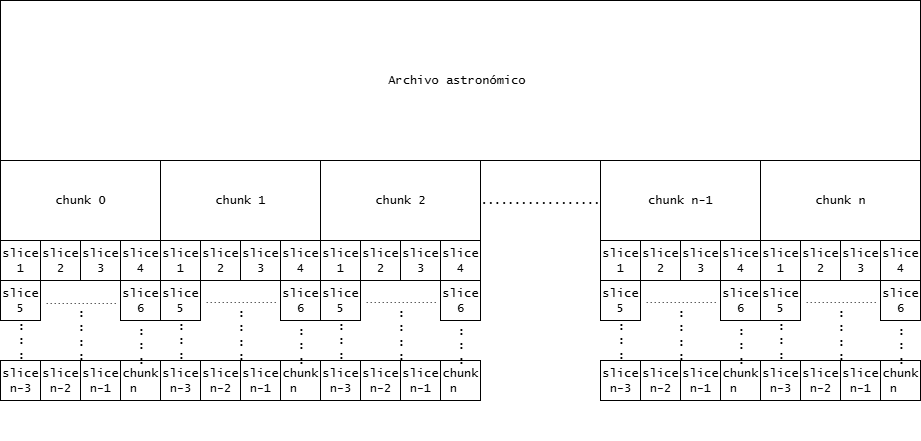
\includegraphics[width=0.9\textwidth]{figures/sistema-chunks.png}
\caption[Esquema de chunks y slices]{Esquema de un archivo astronómico dividido en chunks y slices, ilustrando el concepto de procesamiento con solapamiento. Fuente: Elaboración propia.}
\label{fig:sistema-chunks}
\end{figure}

\subsubsection{Detección y clasificación integradas}
\paragraph{Propuesta de candidatos con CenterNet}
\paragraph{Clasificación binaria en flujo}
\paragraph{Validación física y temporal}

\subsubsection{Análisis y métricas}
\paragraph{Evaluación de rendimiento}
\paragraph{Métricas de calidad y completitud}

\subsubsection{Visualización y artefactos de salida}
\paragraph{Productos diagnósticos estandarizados}
\paragraph{Sistema de logging y auditoría}
\paragraph{Artefactos de salida reproducibles}

\subsubsection{Gestión de configuración y recursos}
\paragraph{Configuración centralizada y validada}
\paragraph{Gestión inteligente de memoria y GPU}
\paragraph{Orquestación y control de flujo}